% ============================================================
% EXPANDED & ANNOTATED VERSION FOR CRITICAL REVIEW
% Original: "Topological Validation of Midsurface Computations"
%           CAD & Applications, 2015
%
% ANNOTATION LEGEND:
%   % [AT-n]   Algebraic Topology deviation / gap (numbered per review plan)
%   % [MR-n]   Mathematical Rigor issue
%   % [NEW]    Proposed new content (section, paragraph, equation)
%   % [FIX]    Correction to existing content
%   % [REF]    Missing or updated reference suggestion
%   % [STYLE]  Writing / presentation issue
% ============================================================

% [STYLE] Current journal class (CADandA) uses 9pt two-column.
% For NeurIPS/SIAM-level submission switch to appropriate class.
% Keeping article class here for readability of annotations.

\documentclass[11pt,a4paper]{article}

% ---- Packages ----
\usepackage[T1]{fontenc}
\usepackage[utf8]{inputenc}
\usepackage{amsmath,amssymb,amsthm}   % [NEW] Essential for proper AT formalism
\usepackage{mathtools}                 % [NEW] Extended math tools
\usepackage{graphicx}
\usepackage{adjustbox}
\usepackage{caption}
\usepackage{booktabs}
\usepackage{enumitem}
\usepackage{hyperref}
\usepackage[margin=1.2in]{geometry}
\usepackage{xcolor}
\usepackage{authblk}
\usepackage{changes}                   % For \added, \replaced markers from original

% ---- Theorem environments (NEW - needed for AT rigor) ----
% [NEW] These environments are required for a mathematically rigorous paper.
% Theorems, lemmas, and proofs should replace the current informal
% "it is evident that" style of validation.
\newtheorem{theorem}{Theorem}[section]
\newtheorem{lemma}[theorem]{Lemma}
\newtheorem{proposition}[theorem]{Proposition}
\newtheorem{corollary}[theorem]{Corollary}
\newtheorem{definition}[theorem]{Definition}
\newtheorem{remark}[theorem]{Remark}

% ---- Notation shorthands (NEW) ----
% [NEW] Define consistent notation for homology groups throughout.
\newcommand{\Hk}[1]{H_{#1}}           % Homology group H_k
\newcommand{\Betti}[1]{\beta_{#1}}    % Betti number beta_k
\newcommand{\Euler}{\chi}             % Euler characteristic
\newcommand{\bdry}{\partial}          % Boundary operator
\newcommand{\Ck}[1]{C_{#1}}          % Chain group C_k
\newcommand{\Zk}[1]{Z_{#1}}          % Cycle group Z_k
\newcommand{\Bk}[1]{B_{#1}}          % Boundary group B_k

% ============================================================
\begin{document}

% ============================================================
% TITLE
% [NEW] Proposed expanded title to signal algebraic topology contribution.
% Original title: "Topological Validation of Midsurface Computations"
% ============================================================
\title{%
  \textbf{Algebraic Topological Validation of Midsurface Abstractions\\
  for Thin-Walled Solids}\\[4pt]
  % [STYLE] Subtitle makes the AT contribution explicit; needed for
  % positioning vs. purely geometric validation papers.
  \large A Homological Framework for Dimension-Reduction Verification
}

\author[1]{Yogesh Kulkarni}
% [NEW] Consider adding a co-author with strong AT background for
% NeurIPS/SIAM submission — the homology sections require expert review.
\affil[1]{Department of Mechanical Engineering, College of Engineering Pune (COEP),
          Pune, India}

\date{
  % [NEW] Add acknowledgement of funding/institution here.
  % [NEW] Add correspondence email.
}

\maketitle
\thispagestyle{empty}

% ============================================================
% ABSTRACT
% ============================================================
\begin{abstract}
% [STYLE] Original abstract is 3 sentences (84 words). A NeurIPS/SIAM
% abstract should be 150-250 words clearly stating: problem, gap,
% method, key result, and significance.

% --- ORIGINAL TEXT (preserved) ---
During the initial stages of the iterative design process, a quick
CAE (Computer-Aided Engineering) analysis of CAD (Computer-Aided Design)
models is needed. To reduce computational resources and time, models are
often simplified by removing irrelevant details and abstracted by reducing
dimension wherever appropriate. Thin-walled parts, such as sheet metal parts,
are often abstracted to a set of surfaces lying midway, called the
\emph{midsurface}. The midsurface is expected to mimic the shape of the
original solid, both geometrically and topologically. Widely-used methods
for assessing midsurface quality are geometric: Hausdorff distance from the
midsurface to its original solid is computed to find gaps and medialness.
Accuracy of such methods depends on sampling as well as on the complexity of
the surface representation, making them computationally intensive and
error-prone.

This paper provides a topological method for verification that is
computationally simple and robust. A novel topological transformation
relationship has been derived between a sheet metal part (solid) and its
midsurface (surface), in both directions (solid-to-surface and
surface-to-solid), which can be used to compare predicted vs.\ actual
entities. Simple as well as practical shapes have been tested to prove the
efficacy of the newly-derived formulation.

% [NEW] ADD the following paragraph to the abstract:
%
% "We ground the transformation rules within the framework of algebraic
% topology: the solid and midsurface are treated as CW complexes, and the
% dimension-reduction map is shown to induce a chain map between their
% respective chain complexes. The Euler characteristic, expressed as the
% alternating sum of Betti numbers, serves as the primary topological
% invariant. We further identify the limitations of single-invariant
% validation and outline an extension based on persistent homology that
% provides a complete topological fingerprint robust to geometric
% perturbations. Experiments on sheet metal benchmarks demonstrate that
% topological validation detects structural midsurface errors --- missing
% surfaces, spurious connections, and incorrect genus --- in O(n) time,
% compared to O(n^2) sampling required by Hausdorff-based methods."

\noindent\textbf{Keywords.} Midsurface, Topological Validation, Euler-Poincar\'e
Equation, Cellular Decomposition, Algebraic Topology, CW Complex, Betti Numbers,
Non-Manifold Topology, Sheet Metal, CAE Simplification.
% [NEW] Add: Homology Groups, Persistent Homology, Chain Complex

\noindent\textbf{DOI} 10.3722/cadaps.2015.xxx-yyy
\end{abstract}

\tableofcontents   % [NEW] Add TOC for expanded version

% ============================================================
\section{Introduction}
% ============================================================

% [STYLE] The introduction currently runs four subsections without
% explicitly stating contributions as a bulleted list. NeurIPS papers
% require a clear, itemised "Contributions" paragraph. Add one after
% the subsections below.

Midsurface is an abstracted representation of a thin-walled solid, used
mainly for creating shell elements in the CAE meshing process. It can also
be used as a shape-signature in shape matching/retrieval. It is expected to
express the contiguous flow of the solid's shape~\cite{Rezayat1996}. So, to
be truly effective, the midsurface needs to mimic the original solid in both
the geometrical and topological sense. Geometrically, the shape of the
midsurface should lie in the middle (at half the thickness) of the solid.
Topologically, the connectivity between the midsurface patches should be
similar to that of their corresponding sub-shapes in the original solid.

There are a large number of methods to compute the midsurface. They work on
different input types of the original solid, such as faceted mesh, Boundary
Representation (Brep) solids, feature-based CAD models, etc. Quality of the
output midsurface depends on the shape characteristics of the original
thin-walled solid.

% [NEW] Insert here: a motivating figure showing a solid, its midsurface,
% and the two validation directions (solid->surface, surface->solid) as a
% pipeline diagram. Something like:
%   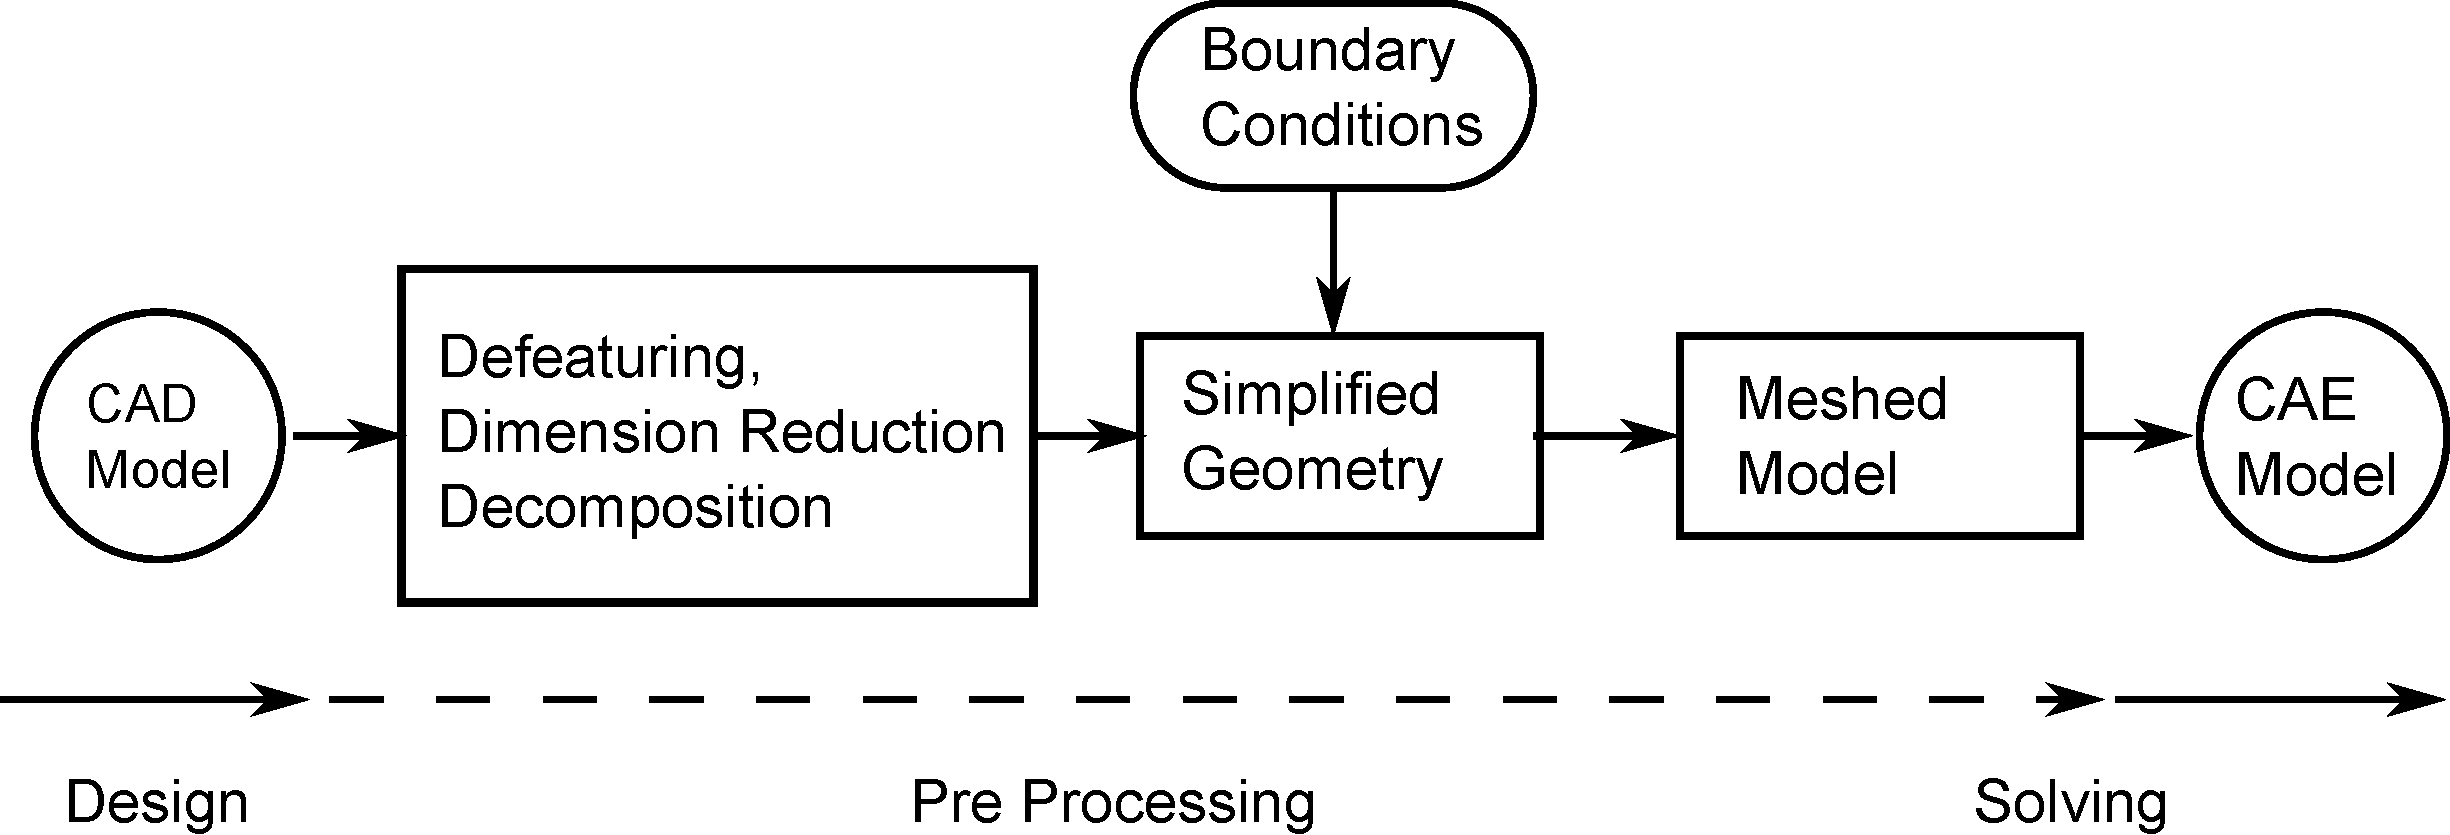
\includegraphics[width=\linewidth]{../Common/images/CADCAEGeneralProcess.pdf}
% with a caption explaining the role of topological validation in the pipeline.

\subsection{Thin-Walled Solids}

Many thin-walled solids come from the sheet metal domain. These are unique
in both the geometrical and topological sense. They are characterized by:

\begin{itemize}[noitemsep,topsep=2pt,parsep=2pt,partopsep=2pt,leftmargin=*]
\item \textbf{Constant thickness}: Sheet metal parts are made from a
      constant-thickness blank roll.
\item \textbf{Absences}: There are no blind holes, only through holes, if any.
\item \textbf{Degeneracy}: There are no degenerate capping thickness faces
      (like a ``Wedge'').
\item \textbf{Cavities}: There are no embedded volumes or cavities (``bubbles'').
\end{itemize}

% [AT-4] DEVIATION: These four characteristics are stated informally but
% are, in fact, topological constraints on the CW-complex structure of the
% solid. They should be formalised as follows (NEW proposed text):
%
% \begin{definition}[Sheet Metal Solid]
% A \emph{sheet metal solid} $\mathcal{S}$ is a compact 3-manifold-with-boundary
% whose CW-complex structure satisfies:
%   (i)  Every 3-cell has exactly two principal 2-cell faces parallel to the
%        blank plane (constant thickness constraint).
%   (ii) Every 2-cell hole is a through-hole: it punctures both principal faces
%        (no blind holes), so it contributes equally to H_1 of the solid and
%        H_1 of the midsurface.
%   (iii) No 2-cell is degenerate (zero-area); all 3-cells are non-degenerate.
%   (iv)  \beta_2(\mathcal{S}) = 1 (one enclosed volume, no bubbles).
% \end{definition}
%
% This definition makes constraint (ii) directly connect to Betti number
% predictions in Section 6, which is currently missing from the paper.

Quality of the output midsurface depends on the complexity of the original
solid. The topological validation method developed in this work has been
devised for solids exhibiting sheet metal shape characteristics. Such
thin-walled solids, with constant thickness, pose fewer problems in both the
computation and validation of the midsurface than those with variable
thicknesses. Although the validation method is derived for constant-thickness
solids, it can be extended to thin-walled parts with variable thickness, e.g.,
injection-moulded plastic parts with drafts. Shapes with or without draft
angles are topologically the same, so the formulation applies equivalently.

% [AT-4] CORRECTION: "Topologically the same" is imprecise. Draft angles
% change the geometry but not the homeomorphism type of the solid, since a
% drafted face is still homeomorphic to a rectangle (disk). The correct
% statement is: "Draft angles constitute a homotopy of the embedding of the
% boundary 2-cells in R^3 but do not change the abstract CW-complex
% structure; hence all homological invariants are preserved."

Many commercial sheet metal CAD modellers represent the thin-walled shape
using a data structure called Boundary Representation (Brep). Section 2
provides the characteristics of Brep and its classification into manifold
and non-manifold representations. In this work, the term `manifold' refers
to an object that is bounded, closed and homeomorphic to a topological sphere
(also known as a 2-manifold), whereas a `non-manifold' object does not have
such restrictions of closure and completeness.

% [AT-1] DEVIATION: The term "2-manifold" is used loosely. In standard
% algebraic topology, a closed 2-manifold is a compact surface without
% boundary. A solid (3D body) is bounded by a closed 2-manifold but is itself
% a 3-manifold-with-boundary. The midsurface is a 2-complex that may NOT
% be a manifold at junction edges (T, Y junctions). These distinctions
% matter when computing homology. The paper should use:
%   - "manifold solid" to mean a 3-manifold-with-boundary whose boundary
%     is a closed 2-manifold.
%   - "non-manifold surface" to mean a 2-complex with singular points
%     (radial edges where more than 2 faces meet).

\subsection{Midsurface Computation}

Midsurface computation has been a widely-researched topic with many methods
such as Medial Axis Transform, Chordal Axis Transform, and Midsurface
Abstraction~\cite{Thakur2009}. Out of these, very few are based on explicit
shape transformation operators.

Sheen et al.~\cite{Sheen2008} used the deflation process to compute a
midsurface from a solid. Their algorithm did not change the topology but
simply reduced capping entities to zero size. The problem with such an
approach is that the degenerated topology would be potentially detrimental
to downstream modelling operations.

Lee~\cite{Lee2009a} proposed topological operators to transform a sheet of
solid topology into a thin-walled solid by face geometry replacement.
However, this method could pose difficulty in representing adjacency
relationships.

% [REF] MISSING: Recent neural-network-based midsurface computation
% methods should be cited here (post-2015 work):
%
% - Kulkarni (2025), "MidcurveNN: Neural Network Approaches for Midcurve
%   Computation," [this group's own work - directly relevant]
% - Koch et al. (2019), "ABC: A Big CAD Model Dataset for Geometric Deep
%   Learning," NeurIPS — establishes the deep-learning CAD context.
% - Sharma et al. (2020), "CSGNet: Neural Shape Parser for Constructive
%   Solid Geometry," CVPR — shape abstraction via ML.
% These papers motivate WHY automated topological validation is needed:
% NN outputs cannot be trusted geometrically; topological checks catch
% structural errors before expensive FEA mesh generation.

Even after extensive research in the academic domain and wide commercial
availability, midsurface quality is still a concern. It suffers from errors
like gaps, overlaps, and missing surfaces. Validating the output midsurface
is a critical step in assessing quality, after which corrective actions can
be taken.

\subsection{Midsurface Validation}

To verify the quality of the midsurface, the following methods are used:

\begin{itemize}[noitemsep,topsep=2pt,parsep=2pt,partopsep=2pt]
\item \textbf{Manual}: Manual inspection for errors such as missing surfaces,
      connection gaps, overlaps, etc. This method is tedious, time-consuming
      and error-prone.
\item \textbf{Inspection Tools}: Tools provided in CAD-CAE packages can
      detect gaps and overlaps but cannot detect correctness at critical
      locations such as connections and steps.
\item \textbf{Geometric Tools}: Hausdorff distance from the midsurface to its
      original solid is computed. Accuracy depends on sampling as well as on
      the complexity of the surface representation, making them computationally
      intensive and error-prone.
\item \textbf{Topological Validation}: Comparison of the number of predicted
      topological entities with actual ones. If there is a mismatch, the
      problem is detected. Geometry is ignored, giving an advantage over
      geometric validation since computationally intensive distance calculations
      are not performed.
\end{itemize}

% [MR-5] MISSING: A complexity comparison table should appear here:
%
% \begin{table}[h]
% \centering
% \begin{tabular}{lll}
% \toprule
% Method & Complexity & Detects \\
% \midrule
% Manual inspection       & O(f) human    & All errors (subjective) \\
% CAD inspection tools    & O(e^2)        & Gaps, overlaps only \\
% Hausdorff distance      & O(n^2)        & Geometric deviation \\
% Topological (this work) & O(f+e+v)      & Structural errors \\
% Homological (proposed)  & O(f+e+v)      & Structural + connectivity \\
% \bottomrule
% \end{tabular}
% \caption{Comparison of midsurface validation methods.}
% \end{table}
%
% where n = number of sample points, f/e/v = faces/edges/vertices.
% The O(f+e+v) claim for topological validation is a key selling point
% that must be formally derived in Section 10.

This work proposes a novel method for the topological validation of the
midsurface of thin-walled solids.

\subsection{Topological Validation}

Topological validation proposed in this work consists of two transformations
with which the quality of a midsurface can be assessed.
\begin{enumerate}
\item \textbf{Solid-to-Surface}: Dimension-reduction transformation equations
      are applied to the thin-walled solid to predict the topological entities
      of the corresponding midsurface. These are then compared with the actual
      topological entities of the output midsurface.
\item \textbf{Surface-to-Solid}: Dimension-addition transformation equations
      are applied to the output midsurface to predict the topological entities
      of the corresponding thin-walled solid. These are then compared with the
      actual topological entities of the thin-walled solid.
\end{enumerate}

% [AT-7] CRITICAL GAP: The paper never states that topological validation
% is a NECESSARY but NOT SUFFICIENT condition for midsurface correctness.
% Add the following remark (essential for mathematical honesty):
%
% \begin{remark}[Necessity vs.\ Sufficiency]
% Topological validation via the Euler characteristic is a \emph{necessary}
% condition for a valid midsurface: any incorrect midsurface that changes
% the topological structure of the solid will fail the check. However, it
% is \emph{not sufficient}: two topologically distinct spaces may share the
% same Euler characteristic (e.g., a torus and a Klein bottle both have
% $\chi = 0$). Therefore, passing the Euler-Poincar\'e check guarantees
% only that the \emph{alternating count} of entities is consistent, not
% that the full topological type is correct.
%
% A stronger sufficient condition can be obtained by verifying that the
% individual Betti numbers $(\beta_0, \beta_1, \beta_2)$ match their
% predicted values --- see Section 8. A complete topological certificate
% requires comparing full homology groups $H_0, H_1, H_2$ --- see Section 9.
% \end{remark}

The validation method presented in this work cannot be used in isolation from
geometry. As the midsurface is applicable only for thin-walled solids, it is
not computed and validated using this method for thick solids. But such
differentiation --- thick or thin --- is \emph{geometrical} and not
\emph{topological}, which this method itself cannot detect. So, the work
presented below should be used only for known thin-walled solids for which
midsurfaces are computable.

Use of topology for assessing the quality of midsurfaces is not widespread
and very few such attempts are reported in the literature.

Lipson~\cite{Lipson} stated that a topological invariant for all sheet metal
parts and thin-walled objects can be used as a necessary condition for
topological validity and reasoning.

Lockett and Guenov~\cite{Lockett2008} used both geometric and topological
variants for checking the validity of the midsurface. For geometric
validation, they used the Hausdorff distance between a midsurface and its
corresponding principal faces. For topological validation, they used proximity
groups adjusted by an angle criterion. The main limitation of their approach
is that geometric criteria (closest distance or angle between faces) are used
in the topological validations, which, ideally, should not be the case.

% [REF] MISSING: The following should be cited and compared here:
%
% - Edelsbrunner, H. and Harer, J. (2010). "Computational Topology: An
%   Introduction." AMS. -- The definitive textbook; justifies using
%   homology rather than just Euler characteristic for shape validation.
% - Dey, T.K. and Wang, Y. (2022). "Computational Topology for Data
%   Analysis." Cambridge University Press. -- Modern reference for TDA.
% - Zomorodian, A. and Carlsson, G. (2005). "Computing Persistent Homology."
%   Discrete & Computational Geometry, 33(2), 249-274. -- Foundation for
%   persistent homology extension proposed in Section 9.
% - Tierny, J. et al. (2017). "The Topology ToolKit." IEEE TVCG. -- Open
%   source TDA for 3D shapes; directly applicable to Brep validation.

Apart from CAE, skeletal structures such as midsurface are used in CAD model
comparison solutions such as shape-based retrieval, similarity assessment and
difference identification~\cite{Antoine2014}. Skeletal graph matching is one
of the prominent techniques~\cite{Iyer2005} for similarity assessment. A
topologically valid midsurface represents sub-shape connectivities better and
thus acts as a more effective shape-signature in model comparison.

The work presented here provides transformation relations and a topological
invariant, based purely on combinatorial topology, for determining the validity
of a midsurface computed from a sheet metal part.

% [O-1] IMPORTANT CORRECTION: The claim "based purely on combinatorial
% topology" is not entirely accurate. The classification of solid cells
% into sCell_{3,0}, sCell_{3,1}, sCell_{3,2}, etc. (by number of touching
% sides) requires geometric adjacency detection. Adjacency is a topological
% concept, but detecting WHICH faces are "touching" in a given decomposition
% requires geometric proximity or Boolean intersection tests.
% Change "purely on combinatorial topology" to "primarily on combinatorial
% topology, with geometric input limited to the cellular adjacency graph."

% ---- NEW: Contributions Paragraph ----
% [NEW] Add the following "Contributions" paragraph at the end of the
% Introduction. This is mandatory for NeurIPS/SIAM-level papers.
%
% \subsection*{Contributions}
% The main contributions of this paper are:
% \begin{enumerate}
%   \item \textbf{Dimension-reduction transformation (solid to midsurface)}:
%         A complete set of rules mapping each cellular component of a
%         sheet metal solid to its midsurface counterpart, with an independent
%         verification that the predicted entities satisfy the non-manifold
%         Euler-Poincar\'e equation.
%   \item \textbf{Dimension-addition transformation (midsurface to solid)}:
%         Inverse transformation rules enabling prediction of solid topology
%         from a classified midsurface, verified against the manifold
%         Euler-Poincar\'e equation.
%   \item \textbf{Formal CW-complex interpretation} (new in this expanded
%         version): Grounding the cellular decomposition in the language of
%         CW complexes and showing the transformation induces a chain map.
%   \item \textbf{Homological validation criterion} (new): Using individual
%         Betti numbers $(\beta_0, \beta_1, \beta_2)$ rather than only the
%         Euler characteristic as validation invariants.
%   \item \textbf{Error taxonomy}: Classification of midsurface errors by
%         whether they are detectable by $\chi$-only, Betti-number, or
%         full-homology validation.
% \end{enumerate}

% ============================================================
% [NEW] SECTION 2: ALGEBRAIC TOPOLOGY BACKGROUND
% ============================================================
% [NEW] This entire section is proposed as new. It is essential for:
% (a) Making the paper self-contained at NeurIPS level.
% (b) Grounding Sections 3-7 in rigorous AT language.
% (c) Bridging the CAD community with AT concepts.
%
% \section{Algebraic Topology Background}\label{sec_at_background}
%
% This section reviews the algebraic topology concepts used throughout
% the paper. Readers familiar with homology theory may skip to Section 3.
%
% \subsection{Simplicial and CW Complexes}
% A \emph{CW complex} $X$ is a topological space built inductively by
% attaching $k$-cells $e^k \cong \mathbb{R}^k$ via attaching maps
% $\phi_k: S^{k-1} \to X^{k-1}$, where $X^{k-1}$ is the $(k-1)$-skeleton.
% The Boundary Representation of a solid and its derived midsurface are
% naturally modelled as CW complexes:
% \begin{itemize}
%   \item 0-cells: vertices $v$
%   \item 1-cells: edges $e$
%   \item 2-cells: faces $f$
%   \item 3-cells: solid volumes (for the manifold solid only)
% \end{itemize}
% The key property we use is that CW complexes admit a well-defined
% chain complex and hence homology groups.
%
% \subsection{Chain Complexes and Boundary Operators}
% For a CW complex $X$, the \emph{$k$-th chain group} $\Ck{k}(X;\mathbb{Z})$
% is the free abelian group generated by the oriented $k$-cells of $X$.
% The \emph{boundary operator} $\bdry_k: \Ck{k} \to \Ck{k-1}$ sends each
% $k$-cell to the signed sum of the $(k-1)$-cells on its boundary.
% These fit into the \emph{chain complex}:
% $$\cdots \xrightarrow{\bdry_{k+1}} \Ck{k} \xrightarrow{\bdry_k} \Ck{k-1}
%   \xrightarrow{\bdry_{k-1}} \cdots \xrightarrow{\bdry_1} \Ck{0}
%   \xrightarrow{\bdry_0} 0$$
% with the fundamental property $\bdry_{k-1} \circ \bdry_k = 0$.
%
% \subsection{Homology Groups}
% The \emph{$k$-th homology group} is defined as:
% $$\Hk{k}(X) = \Zk{k}(X) / \Bk{k}(X)$$
% where $\Zk{k} = \ker \bdry_k$ (cycles) and $\Bk{k} = \operatorname{im} \bdry_{k+1}$
% (boundaries). The rank of $\Hk{k}$ is the \emph{$k$-th Betti number}
% $\Betti{k} = \operatorname{rank} \Hk{k}$.
% Intuitively:
% \begin{itemize}
%   \item $\Betti{0}$: number of connected components.
%   \item $\Betti{1}$: number of independent loops (handles, tunnels).
%   \item $\Betti{2}$: number of enclosed voids (cavities).
% \end{itemize}
%
% \subsection{Euler Characteristic as Alternating Sum of Betti Numbers}
% For any finite CW complex $X$ of dimension $D$:
% $$\Euler(X) = \sum_{k=0}^{D} (-1)^k N_k = \sum_{k=0}^{D} (-1)^k \Betti{k}$$
% where $N_k$ is the number of $k$-cells. This is the Euler-Poincar\'e
% theorem. It implies that $\Euler$ is a WEAKER invariant than the full
% sequence $(\Betti{0}, \Betti{1}, \ldots, \Betti{D})$: many different
% Betti-number combinations can yield the same $\Euler$.
%
% \textbf{Consequence for validation}: Checking only $\Euler$ (as done in
% the current paper) will miss errors where individual Betti numbers change
% but their alternating sum is preserved. Example: a midsurface that gains
% one spurious loop ($\beta_1 \uparrow 1$) AND one spurious void ($\beta_2
% \uparrow 1$) has the same $\chi$ but different topology.
%
% \subsection{Chain Maps and Induced Homomorphisms}
% A \emph{chain map} $f_*: (C_*(X), \bdry) \to (C_*(Y), \bdry)$ is a
% collection of group homomorphisms $f_k: \Ck{k}(X) \to \Ck{k}(Y)$
% commuting with boundary operators:
% $$f_{k-1} \circ \bdry_k^X = \bdry_k^Y \circ f_k$$
% Chain maps induce homomorphisms on homology: $f_*: \Hk{k}(X) \to \Hk{k}(Y)$.
%
% [AT-4] The dimension-reduction map (solid $\to$ midsurface) proposed in
% Section 5 should be proven to be a chain map. If it is, the induced
% homomorphisms on homology give the exact predicted Betti numbers of the
% midsurface. Currently the paper only checks the alternating sum (Euler
% characteristic), missing the richer information in the individual
% $\Hk{k}$ maps.

% ============================================================
\section{Preliminaries}\label{sec_preliminaries}
% ============================================================

% [STYLE] The original paper merges "Background" and "Preliminary"
% material into a section called "Preliminaries." With the new AT
% Background section (Section 2 above), this section should be
% retitled "Boundary Representation and Euler-Poincar\'e Equations"
% and streamlined to focus on Brep-specific AT.

\subsection{Boundary Representation (Brep)}

Brep is composed of two parts: topology and geometry. Topological elements
are shells, faces, edges, vertices, etc., listed in descending order of
topological dimensionality:

\begin{itemize}[noitemsep,topsep=2pt,parsep=2pt,partopsep=2pt]
\item \emph{shell (s)}: a connected set of \emph{faces}
\item \emph{face (f)}: a bounded portion of a \emph{surface} (geometry)
\item \emph{loop (l)}: a circuit of \emph{edges} bounding a \emph{face}
\item \emph{half-edges (he)}: used to create a \emph{loop}
\item \emph{edge (e)}: a bounded portion of a \emph{curve} (geometry)
\item \emph{vertex (v)}: lies at a \emph{point} (geometry)
\end{itemize}

% [NEW] Add the following to connect Brep to CW-complex language:
%
% \begin{remark}[Brep as CW Complex]
% The Brep data structure is precisely a CW complex in disguise: vertices
% are 0-cells, edges are 1-cells (with attaching maps to their two endpoint
% vertices), faces are 2-cells (with attaching maps given by their loops),
% and solid volumes are 3-cells. The "loops" in Brep correspond to the
% attaching maps $\phi_2: S^1 \to X^1$ of 2-cells. Inner loops (holes in
% faces) correspond to additional generators of $\Hk{1}$ of that face's
% attaching map, captured by the ring count $r$ in the Euler-Poincar\'e
% equation.
% \end{remark}

Validity of the Brep model is checked using the Euler-Poincar\'e equation.

\subsubsection{Euler-Poincar\'e Equation}

Euler's equation for polyhedral solids is:
\begin{equation}
  v - e + f = 2
\end{equation}
where $v$, $e$, and $f$ represent the number of vertices, edges and faces
respectively. It was discovered by Leonhard Euler in 1752 and was later
generalised by Lhuilier~\cite{Krishnamurti2002}:
\begin{equation}
  v - e + f = 2 - 2g
\end{equation}
where $g$ represents the genus (number of handles). Later, Schl\"afli and
Poincar\'e generalised the formula to higher-dimensional $n$-polytopes.

% [NEW] Add here the DERIVATION of the Euler-Poincar\'e formula from
% first principles using homology:
%
% \begin{theorem}[Euler-Poincar\'e for CW Complexes]
% For any finite CW complex $X$:
% $$\sum_{k \geq 0} (-1)^k N_k = \sum_{k \geq 0} (-1)^k \Betti{k}$$
% \begin{proof}[Proof sketch]
% By the rank-nullity theorem applied to each boundary operator:
% $N_k = \operatorname{rank}(\Bk{k}) + \operatorname{rank}(\Zk{k})$
% and $\Betti{k} = \operatorname{rank}(\Zk{k}) - \operatorname{rank}(\Bk{k-1})$.
% Summing with alternating signs causes the boundary-rank terms to cancel
% in telescoping fashion, yielding the result. $\square$
% \end{proof}
% \end{theorem}
%
% This proof is absent from the current paper but is essential for
% justifying that the formulas in Eqns (1)-(4) are instances of the
% same underlying theorem, not separate ad hoc equations.

The Euler characteristic ($\chi$) for combinatorial cell complexes or
polyhedral solids is defined as:
\begin{equation}
  \sum_{i=0}^{D}(-1)^{i} N_{i}= \sum_{i=0}^{D}(-1)^{i} \beta_{i} = \chi
  \label{eqn_betti}
\end{equation}

For dimensions up to 3 ($i \leq 3$), equation~(\ref{eqn_betti}) simplifies to:
\begin{equation}
  N_{0}-N_{1}+N_{2}= \beta_{0} -\beta_{1} + \beta_{2}
  \label{eqn_betti3}
\end{equation}
where $N$s are topological entities of dimensions 0, 1, and 2 respectively,
and $\beta$s are the Betti numbers. $\beta_{0}$, $\beta_{1}$ and $\beta_{2}$
correspond to the number of connected components, loops and cavities,
respectively~\cite{Sequin}.

% [AT-1] DEVIATION: The paper introduces beta_0, beta_1, beta_2 here but
% then NEVER uses them individually again. The entire validation in
% Sections 4-5 reduces everything to the single number chi. This is a
% fundamental weakness. The expanded paper must:
% (a) Compute predicted Betti numbers (not just chi) for both solid
%     and midsurface.
% (b) State explicitly what each Betti number means for sheet metal:
%     beta_0 = 1 always (one connected solid)
%     beta_1 = number of through-holes h
%     beta_2 = 1 for solid (one enclosed volume), 0 for open midsurface
% (c) Show that the transformation predicts a specific Betti-number
%     signature, not merely the same chi.

Two homeomorphic topological spaces will have the same Euler characteristic
and Betti numbers.

% [AT-2] ADD: Two spaces with the same Euler characteristic need NOT be
% homeomorphic (or even homotopy equivalent). The converse is false.
% This is the soundness gap in using chi as the sole validator.

Most CAD models are made up of solids (manifolds), since they are considered
complete, having their own volumes. A manifold-solid model can only represent
one closed volume minus its internal structure. It cannot represent
heterogeneous possibilities such as wires (curves), sheets (surfaces) and
solids (volumes) together~\cite{Yamaguchi1995}. A non-manifold model is a
generic modelling framework that encompasses all these items in a single
framework~\cite{Lee2001}.

The Euler characteristic $\chi$ in terms of Betti numbers provides a generic
invariant for a shape of any dimension. When a thin-walled solid is
transformed into its corresponding midsurface, the interpretation of the
Betti numbers changes from the manifold domain to the non-manifold domain.

% [AT-5] DEVIATION: The change in Betti-number interpretation across the
% transformation is the CORE of the paper, yet it is stated in one sentence
% and never expanded. The expanded paper should have a subsection:
%
% "3.1.x Betti Numbers: Solid vs Midsurface Interpretation"
% Solid (manifold, closed):
%   beta_0 = s  (shells/components)
%   beta_1 = 2h (twice the genus, since the solid's boundary 2-manifold
%                has 2g independent curves but the solid interior reduces
%                this by h due to each handle being contractible)
%   beta_2 = s  (each closed shell encloses one void)
%
% Midsurface (non-manifold, open):
%   beta_0 = s  (connected components of surface)
%   beta_1 = h  (independent loops on the open surface, each through-hole
%                contributes one loop; no "doubling" because the surface
%                has a boundary)
%   beta_2 = 0  (no enclosed volumes; the midsurface is open)
%
% This mapping (beta_1: 2h -> h) is the key topological change induced
% by the dimension reduction. It is never proven in the current paper.

\subsubsection{Manifold Solids}

The Euler-Poincar\'e equation for manifold solids is:
\begin{equation}
  v - e + (f - r) = 2(s - h)
  \label{eqn_manifold}
\end{equation}

Its equivalence with equation~(\ref{eqn_betti3}) is as follows:

\begin{itemize}[noitemsep,topsep=2pt,parsep=2pt,partopsep=2pt,label={}]
\item $N_{0} = v$: number of vertices
\item $N_{1} = e$: number of edges
\item $N_{2} = (f - r)$: number of faces ($f$) minus inner loop artifacts ($r$)
\item $\beta_{0} = s$: number of shells (connected components)
\item $\beta_{1} = 2h$: number of independent closed curves (twice genus $h$)
\item $\beta_{2} = s$: number of enclosed regions
\end{itemize}

% [AT-5] CLARIFICATION NEEDED: The statement beta_1 = 2h for a SOLID is
% incorrect in general. For a solid 3-manifold-with-boundary bounded by a
% genus-g surface, beta_1 of the solid = g (NOT 2g), because half the
% generators of pi_1 of the boundary are null-homologous in the interior.
% (This is a consequence of the half-lives/half-dies lemma from 3-manifold
% topology.) The factor of 2 appears for the BOUNDARY SURFACE, not the solid.
%
% The equation 2(s-h) on the RHS of Eq. 3 conflates:
%   - The genus of the boundary surface (2h)
%   - The beta_2 = s contribution (number of shells)
% into one expression. This is correct numerically (as the formula is
% standard in CAD literature, cf. Mantyla 1988) but is presented without
% justification. Add a footnote or remark clarifying this subtlety.

\subsubsection{Non-Manifold Surfaces}

Solids found in the real world have the property that at any point on the
boundary, a small enough sphere at that location is split into exactly two
pieces, one inside and one outside the object. Non-manifolds do not obey this
rule~\cite{Krishnamurti2002}. Weiler~\cite{Weiler1986} made the first
significant contribution in defining the non-manifold data structure, called
the \emph{Radial Edge Structure}. Core to this data structure is the radial
cycle: an ordered list of faces around an edge. Similar to the manifold case,
the equation for non-manifold topology~\cite{Yamaguchi2002} is:

\begin{equation}
  v - e + (f - r) = s - h
  \label{eqn_nonmanifold}
\end{equation}

Its equivalence with equation~(\ref{eqn_betti3}) is as follows:

\begin{itemize}[noitemsep,topsep=2pt,parsep=2pt,partopsep=2pt,label={}]
\item $N_{0} = v$: number of vertices
\item $N_{1} = e$: number of edges
\item $N_{2} = (f - r)$: number of faces minus inner loops
\item $\beta_{0} = s$: number of shells
\item $\beta_{1} = h$: number of independent loops (through-holes)
\item $\beta_{2} = 0$: no enclosed volumes (the surface is open)
\end{itemize}

% [AT-5] FIX: The claim beta_2 = 0 for a non-manifold surface needs
% justification: An open surface (surface with boundary) has H_2 = 0
% because there are no closed 2-cycles (every 2-chain has a boundary).
% This follows from the long exact sequence of the pair (surface, boundary):
%   ... -> H_2(boundary) -> H_2(surface) -> H_2(surface, boundary) -> ...
% Since boundary = 1-manifold (disjoint loops), H_2(boundary) = 0, and
% H_2(surface, boundary) = H^0(surface) by Poincare-Lefschetz duality,
% the argument shows H_2(surface) = 0 for surfaces with nonempty boundary.
% Add this justification as a brief proof or citation.

% [AT-8] GROUNDING NEEDED: "Radial edge" in Weiler's Radial Edge Structure
% corresponds, in AT language, to the "link" of an edge in the CW complex.
% At a manifold edge, the link is a 0-sphere S^0 (two points = two faces).
% At a non-manifold (radial) edge, the link has more than two points
% (multiple faces). Formally, an edge $e$ is called "non-manifold" if its
% link lk(e) is not homeomorphic to S^0. This topological definition
% should replace the geometric description currently in the paper.

\subsection{Cellular Decomposition}

Cellular topology is one of the prominent representations in solid modelling.
The fundamental unit is called a \emph{Cell}, with dimensionality $0/1/2/3$,
and can have adjacency to its neighbours denoted as
$\text{Cell}_{\text{dimension},\text{adjacency}}$. The actual size and shape
of cells can vary based on the underlying geometry
(Table~\ref{tbl_celldecompexample}).

\begin{minipage}{0.9\linewidth}
\begin{center}
\begin{tabular}[h]{@{}p{0.22\linewidth} p{0.22\linewidth} | p{0.22\linewidth}
  p{0.22\linewidth}@{}}
\toprule
{\bf Original Part} & {\bf Cellular Model} & {\bf Original Part} & {\bf Cellular Model} \\
\midrule
\adjustbox{valign=t}{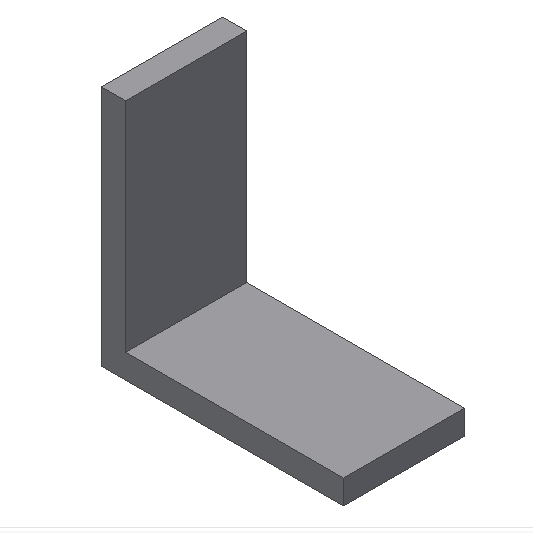
\includegraphics[width=0.8\linewidth]{../Common/images/nonCellularL}} &
\adjustbox{valign=t}{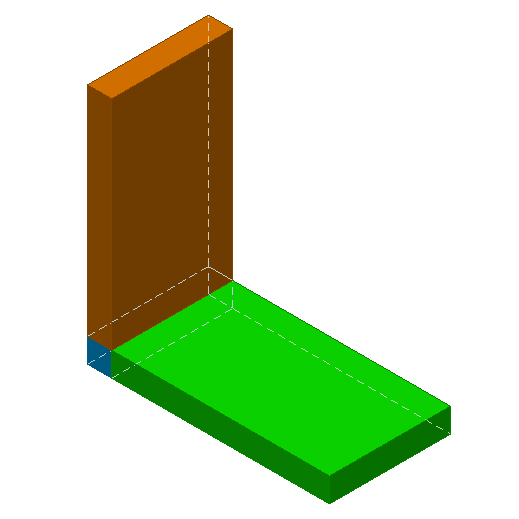
\includegraphics[width=0.8\linewidth]{../Common/images/CellularL}} &
\adjustbox{valign=t}{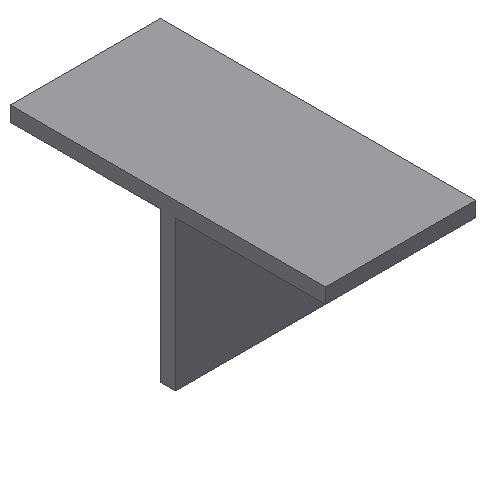
\includegraphics[width=0.8\linewidth]{../Common/images/nonCellularT}} &
\adjustbox{valign=t}{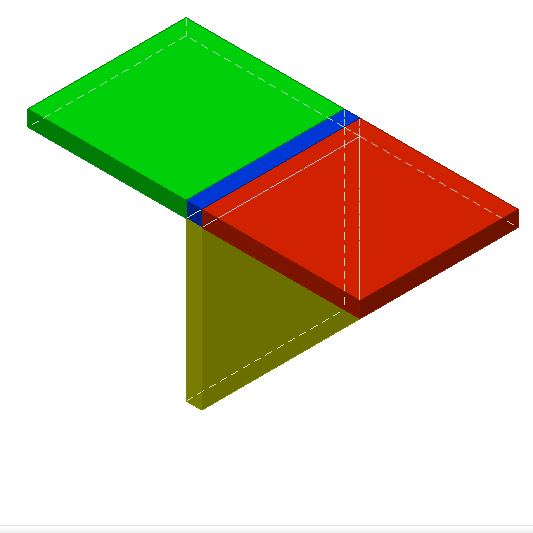
\includegraphics[width=0.8\linewidth]{../Common/images/CellularT}} \\
\midrule
\adjustbox{valign=t}{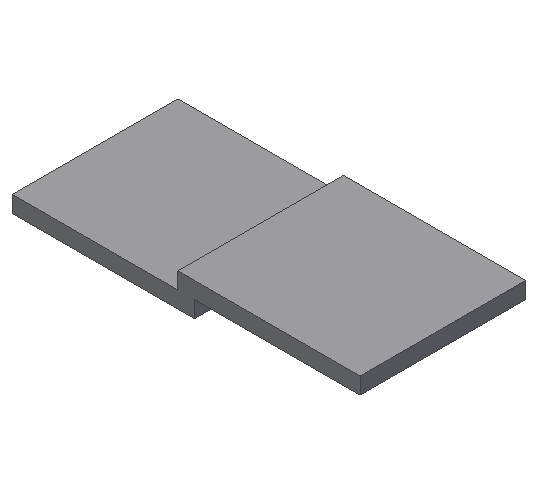
\includegraphics[width=0.8\linewidth]{../Common/images/nonCellularOverlap}} &
\adjustbox{valign=t}{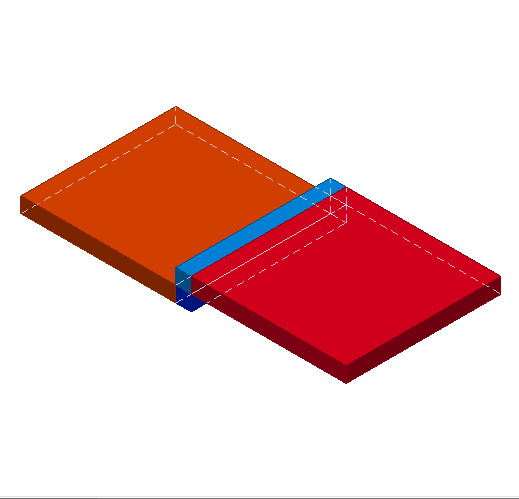
\includegraphics[width=0.8\linewidth]{../Common/images/CellularOverlap}} &
\adjustbox{valign=t}{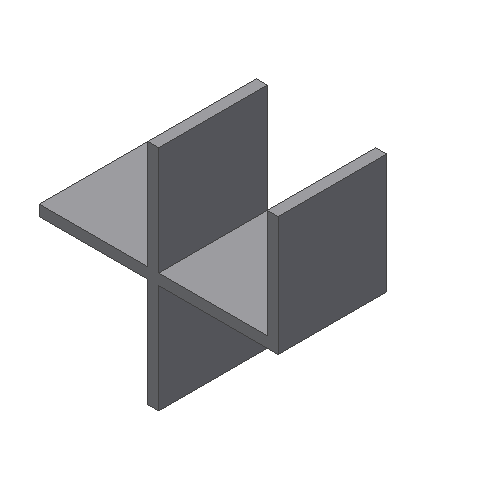
\includegraphics[width=0.8\linewidth]{../Common/images/nonCellularZU}} &
\adjustbox{valign=t}{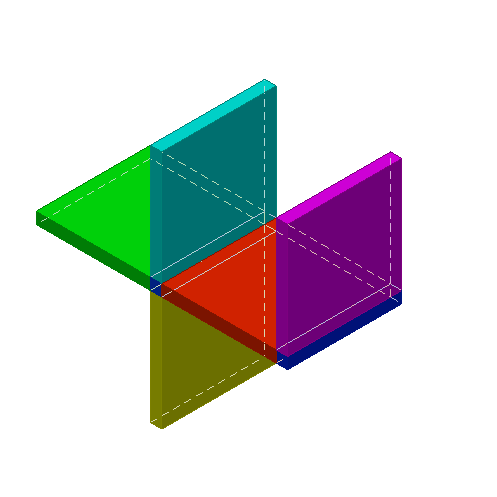
\includegraphics[width=0.8\linewidth]{../Common/images/CellularZU}} \\
\bottomrule
\end{tabular}
\captionof{table}{Decomposition of shapes into Cells}
\label{tbl_celldecompexample}
\end{center}
\end{minipage}

% [NEW] Add the following CW-complex interpretation:
%
% \begin{remark}[Cellular Decomposition as a CW Complex]
% The cellular decomposition described here is precisely a CW complex
% construction on the solid $\mathcal{S}$. Each sCell$_{3,n}$ is a
% 3-cell attached to the 2-skeleton (the bounding faces). Each
% iCell$_{3,n}$ and iCell$_{2,2}$ are interface cells created by
% intersections between adjacent solid cells; they correspond to the
% attaching maps between 3-cells sharing a common 2-face. The resulting
% decomposed complex $\mathcal{S}_\Delta$ is a CW complex with the same
% homotopy type as $\mathcal{S}$ (the decomposition does not change the
% topology of the solid). This invariance is a necessary condition for
% the transformation rules in Section 5 to be well-defined: the predicted
% midsurface topology must be independent of the choice of decomposition.
%
% OPEN PROBLEM: Is the topological validation independent of the
% cellular decomposition chosen? Two different valid decompositions of
% the same solid should yield the same midsurface Betti numbers. This
% claim is NOT proven in the current paper and is a significant gap.
% \end{remark}

\subsubsection{Cellular Entities}

Cellular Decomposition is a process by which a shape (the ``original solid'')
is split into multiple sub-shapes (``Cells''). According to Chen et
al.~\cite{Chen2006}, a cellular model includes topologies of various
dimensions:
$$\mathbb{M} =
  \left(\bigcup_{i=1}^{q} C_i^0 \right) \cup
  \left(\bigcup_{j=1}^{r} C_j^1 \right) \cup
  \left(\bigcup_{k=1}^{s} C_k^2 \right) \cup
  \left(\bigcup_{l=1}^{t} C_l^3 \right)$$
where $C_i^0$ are 0-dimensional vertices, $C_j^1$ are 1-dimensional edges,
$C_k^2$ are 2-dimensional faces and $C_l^3$ are 3-dimensional solids. Cells
have the following properties:

\begin{itemize}[noitemsep,topsep=2pt,parsep=2pt,partopsep=2pt]
\item \textbf{Boundary}: Except $C_i^0$ cells, all cells are bound by cells
      with dimension lower by 1. \emph{[This is precisely the CW complex
      closure condition.]}
\item \textbf{Overlap}: No cells overlap:
      $C_i^a \cap C_j^b = \emptyset$,
      $(0 \leq a, b \leq 3,\; (a = b) \wedge (i \neq j))$
\item \textbf{Nature}: Either additive or subtractive.
\end{itemize}

% [MR-1] INCOMPLETENESS: Are the following the ONLY cell types for
% sheet metal? What about:
% - Cells with n=3 touching sides (e.g., a corner piece in a box)?
% - Cells with n=4 (a completely enclosed piece)?
% The paper never proves this classification is complete.
% Add a COMPLETENESS LEMMA:
%
% \begin{lemma}[Completeness of Cell Classification for Sheet Metal]
% For a sheet metal solid satisfying Definition X (constant thickness,
% no blind holes, no cavities), the cellular decomposition yields only
% cells of the following types: sCell_{3,n} for n in {0,1,2}, sCell_{3,h},
% iCell_{3,n} for n >= 2, and iCell_{2,2}. Cells with n >= 3 solid-side
% contacts do not arise for sheet metal parts (proof: three mutually
% adjacent planar faces in a constant-thickness solid would require the
% part to be at least locally volumetric at the junction, violating the
% thin-wall constraint).
% \end{lemma}
%
% Without this lemma, the transformation rules in Section 5 are not
% proven to cover all cases.

Cells can be of the following types:

\begin{tabular}[h]{@{}p{0.1\linewidth} p{0.1\linewidth} p{0.4\linewidth}
  p{0.4\linewidth}@{}}
\toprule
$\text{Cell}_{3,*}$ &
\adjustbox{valign=t}{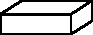
\includegraphics[width=\linewidth]{../Common/images/SimplePlate1.pdf}} &
3D cells (solids), topologically similar to a simple plate &
$f=6,\; e=12,\; v=8$ \\
$\text{Cell}_{2,*}$ &
\adjustbox{valign=t}{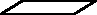
\includegraphics[width=\linewidth]{../Common/images/SimplePlane1.pdf}} &
2D cells, topologically similar to a planar surface &
$f=1,\; e=4,\; v=4$ \\
$\text{Cell}_{1,*}$ &
\adjustbox{valign=t}{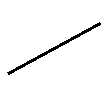
\includegraphics[width=\linewidth]{../Common/images/SimpleLine1.pdf}} &
1D cells, topologically equivalent to a line &
$e=1,\; v=2$ \\
$\text{Cell}_{3,h}$ &
\adjustbox{valign=t}{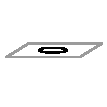
\includegraphics[width=\linewidth]{../Common/images/SimpleHole1.pdf}} &
Hole assumed cylindrical through-all (true for sheet metal) &
$e=1,\; v=1$ \\
\bottomrule
\end{tabular}

% [MR-4] NOTE: The entities for Cell_{3,h} (e=1, v=1) represent the
% loop topology of a through-hole (one circular edge, one virtual vertex).
% This is the standard way to encode an annular topology in Brep.
% However, the paper should clarify: a through-hole in a solid corresponds
% topologically to removing a solid cylinder (D^2 x [0,1]) from the solid,
% which adds one generator to H_1 of the solid (beta_1 increases by 1)
% and correspondingly in the midsurface. The (e=1, v=1) count should be
% derived from the boundary of the cylindrical cut, not stated ad hoc.

\subsubsection{Classification of Cells}

When the original solid is decomposed into distinguishable cells, new
interface boundaries are introduced. Newly-created intersecting volumes or
touching boundaries are called interface-cells, which can be either 3D
(solids) or 2D (faces):

\begin{itemize}[noitemsep,topsep=2pt,parsep=2pt,partopsep=2pt]
\item Two shapes touching with an area-overlap form a 2D interface.
\item Two shapes touching with a volume-overlap form a 3D interface.
\end{itemize}

If two bodies spatially overlap, they are split to form the 3D interface
cell (Fig.~\ref{fig:3dinterface}). In the case of a 2D Interface
(Fig.~\ref{fig:2dinterface}), the adjoining faces are extended~\cite{Woo2002}
and used as a cutting tool to create the 3D Interface cell.

\begin{minipage}[t]{\linewidth}
\centering
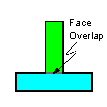
\includegraphics[width=0.4\linewidth]{../Common/images/Interface2d_1.pdf}
\captionof{figure}{2D Interface}
\label{fig:2dinterface}
\end{minipage}

\begin{minipage}[t]{\linewidth}
\centering
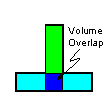
\includegraphics[width=0.4\linewidth]{../Common/images/Interface3d_1.pdf}
\captionof{figure}{3D Interface}
\label{fig:3dinterface}
\end{minipage}

% [MR-4] The two interface types (2D and 3D) ultimately yield the SAME
% midsurface transformation result (e=1, v=2 in both Eqns 5-6). But
% their topological justification differs:
% - A 3D interface cell (volume) reduces to a midsurface edge because
%   a 3D junction region, squeezed to zero thickness, becomes a 1D spine.
% - A 2D interface cell (shared face) reduces to a midsurface edge because
%   two surface patches meeting at a face share that face's midline.
% The paper should derive BOTH cases from the boundary operator formalism,
% not just state the result.

Prefix $s$ is applied if the Cell is from the original solid, $i$ for a
newly-introduced interface type (Fig.~\ref{fig_celldecompexample}), and $m$
for midsurface cells.

\begin{minipage}[t]{\linewidth}
\centering
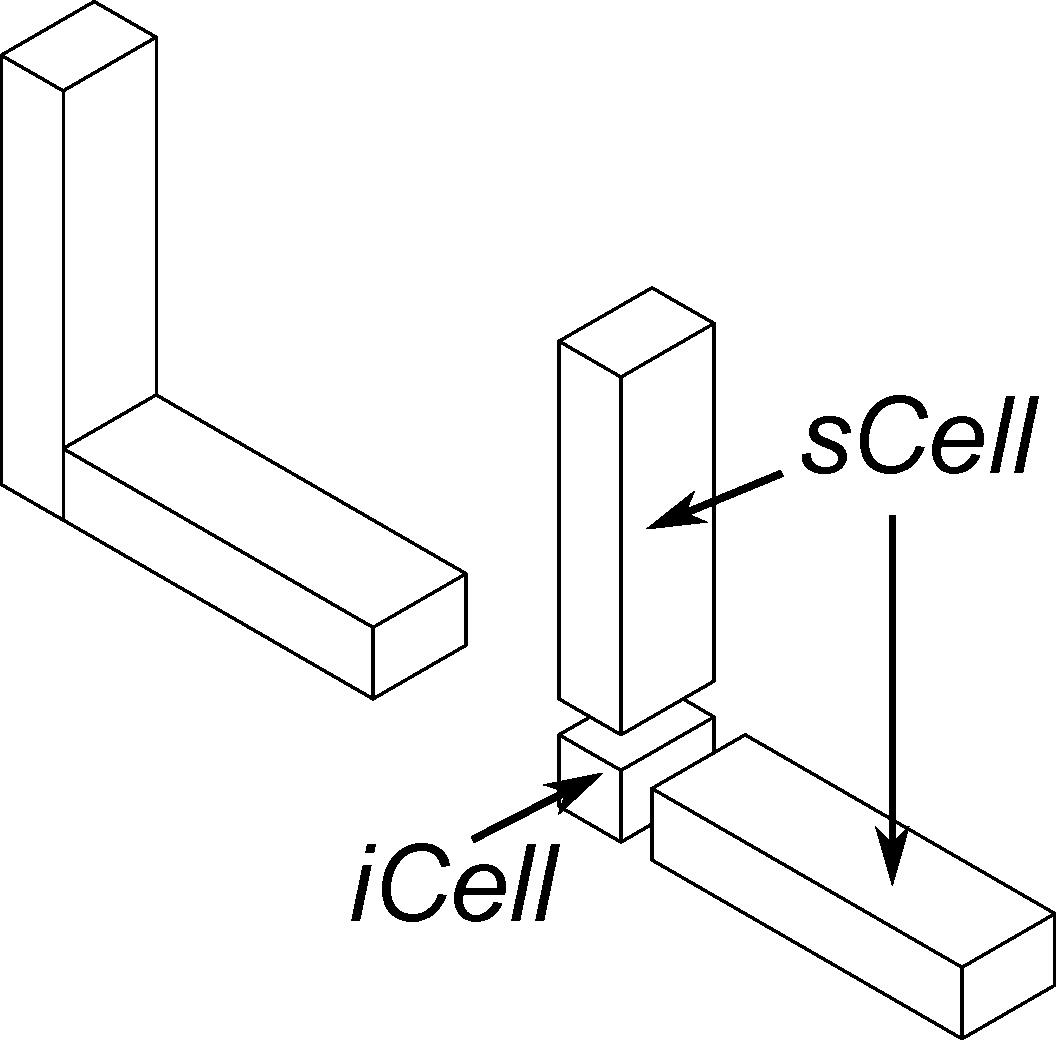
\includegraphics[width=0.6\linewidth]{../Common/images/CellDecompExample}
\captionof{figure}{Decomposition \& classification~\cite{Treeck}}
\label{fig_celldecompexample}
\end{minipage}

% ============================================================
% END OF PART 1 (Sections 1-3)
% Next: Sections 4-7 (Transformations, Examples, Validation)
% ============================================================

% Placeholder for Part 2 (to be appended):
% \input{TopoVal_cadanda_expanded_v1_part2}

\end{document}
